\documentclass[11pt]{article}

\usepackage{default}
\usepackage{fullpage}
\usepackage{fancyhdr}
\usepackage{amsmath}
\usepackage{amssymb}
\usepackage{amsthm}
\usepackage{setspace}
\usepackage{graphicx}
\usepackage{url}
\usepackage{algorithm}
\usepackage{algpseudocode}

\usepackage{tikz}
\usetikzlibrary{arrows,shapes}

\pagestyle{fancy}
\setlength{\headheight}{16pt}
\rhead{\today}

\newcommand{\R}{\mathbb{R}}
\newcommand{\Z}{\mathbb{Z}}

\newcommand{\st}{\mbox{s.t.}}

\DeclareMathOperator*{\argmax}{arg\,max}
\DeclareMathOperator*{\argmin}{arg\,min}
\newtheorem{theorem}{Theorem}

\bibliographystyle{plain}

% Commands for build_A.m variable names
\newcommand{\connections}{\texttt{Connections.xlsx}}
\newcommand{\inputs}{\texttt{Inputs.xlsx}}
\newcommand{\buildA}{\texttt{build\_A.m}}
\newcommand{\A}{\texttt{A}}
\newcommand{\Ast}{\texttt{A\_st}}
\newcommand{\Alag}{\texttt{A\_lag}}

\newcommand{\numUsers}{\texttt{numUsers}}
\newcommand{\numArcs}{\texttt{numArcs}}
\newcommand{\numStorage}{\texttt{numStorage}}
\newcommand{\numRelease}{\texttt{numRelease}}
\newcommand{\numWS}{\texttt{numWS}}
\newcommand{\sw}{\texttt{sw\_row}}
\newcommand{\gw}{\texttt{gw\_row}}

\begin{document}

\section{Connections file \connections}
\label{sec:connectionsxlsx}

The file \texttt{Connections.xlsx} stores the directed water network in a structure designed by Alicia Forrester.
The files stores the network in a 0-1 matrix with a structure similar to a (node-node) adjacency matrix (see, e.g., \url{http://en.wikipedia.org/wiki/Adjacency_matrix}).
However, the structure differs from the standard adjacency matrix in the following ways:
\begin{enumerate}
	\item The rows and columns are reversed from the adjacency matrix.
		I.e., if there is a 1 $i$th row and $j$th column, this indicates an arc from node $j$ to node $i$.
	\item The rows (referred to as \emph{users}) and columns (referred to as \emph{sources}) contain \textbf{only a subset} of the total nodes in the system.
	\begin{enumerate}
		\item Consequently, the $i$th row may represent to a different node than the $i$th column.
		\item Thus, every node must be identified by a unique name.
		\begin{enumerate}
			\item In the MATLAB code, this name must be a string.
			\item Details on which nodes are included as a source is found in Section \ref{ssec:sources}.
			\item Details on which nodes are included as a user is found in Section \ref{ssec:users}.
		\end{enumerate}
		\item Furthermore, this structure ensures that \textbf{some arcs are implied}, i.e., they exist in the network even though they are not shown in the matrix.
	\end{enumerate}
\end{enumerate}

\subsection{Node types}
\label{ssec:nodetypes}

Every node is given a type, represented by a positive integer, describing its role in the water system.
As of this writing, the possibilities are:
\begin{center}
	\begin{tabular}{|l|l|c|}
		\hline
		Type										& Abbreviation		& Number \\
		\hline
		Groundwater Source					& \texttt{GW}		& 1 \\
		Waste Water Treatment Plant		& \texttt{WWTP}	& 2 \\
		Surface Water Source					& \texttt{SW}		& 3 \\
		Water Treatment Plant				& \texttt{WTP}		& 4 \\
		Dummy Source							& \texttt{DMY}		& 5 \\
		Recharge Facility						& \texttt{RCHRG}	& 6 \\
		Potable Interceptor/Reservoir		& \texttt{P}		& 7 \\
		Non-potable Interceptor/Booster	& \texttt{NP}		& 8 \\
		Return Interceptor					& \texttt{RTRN}	& 9 \\
		Potable Municipal User				& \texttt{PMU}		& 10 \\
		Non-potable Municipal User			& \texttt{NPMU}	& 11 \\
		Potable Industrial User				& \texttt{PIN}		& 12 \\
		Non-potable Industrial User		& \texttt{NPIN}	& 13 \\
		Potable Agricultural User			& \texttt{PAG}		& 14 \\
		Non-potable Agricultural User		& \texttt{NPAG}	& 15 \\
		\hline
	\end{tabular}
\end{center}

\subsection{Sources}
\label{ssec:sources}

The sources list contains every node with an outgoing arc, \emph{except nodes where the outgoing arc is implied}.
Every node that does not have a demand associated with it is listed as a source.
Source node names are given in row 1 of \connections, beginning in column D.
Row 2 contains the node type of each source.

\textbf{Node types unique to Sources:}
\begin{itemize}
	\item Groundwater sources
	\item Surface water sources
	\item Dummy sources
\end{itemize}


\subsection{Users}
\label{ssec:users}

The users list contains every node with an incoming arc, \emph{including nodes where the incoming arc is implied}.
User node names are given in column A of \connections, beginning in row 3.
User (elevation) zones are given in column B.
User types are given in column C.

\textbf{Node types unique to Users:}
\begin{itemize}
	\item Potable users of all types (municipal, industrial and agricultural)
	\item Non-potable users of all types
\end{itemize}

\subsection{Implied Outgoing Arcs of Potable Users}
\label{ssec:potableusers}

In a standard minimum cost flow problem, water enters the system at supply nodes and leaves the system at demand nodes.
Non-potable demands in the water model behave in exactly this way.
However, water satisfying potable demands is returned (after some loss) for treatment.
Thus, we need to modify the standard formulation slightly to accommodate the fact that potable demand flows through the nodes.

Figure \ref{fig:demand1} shows a simple setup where two facilities supply potable water to a potable demand source, which then returns waste-water to a return interceptor.
The problem needs a constraint ensuring that the total flow going \emph{through} the demand node \texttt{DemP} meets the potable demand.
Furthermore, we require that all water flowing into \texttt{DemP} be used to satisfy demand, i.e., the total flow into \texttt{DemP} exactly equals the demand.
The code enforces these requirements by changing the system seen in Figure \ref{fig:demand2}.
The flow variables going into \texttt{DemP} are copied (subtracting the loss) and used as inputs in \texttt{RTRN}.
Now, flow from \texttt{P} and \texttt{IPR} satisfy demand at \texttt{DemP}, given in the right hand side vector.

\begin{figure}[ht]
	\centering
	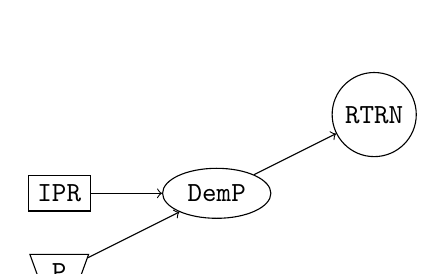
\begin{tikzpicture}
		\node[draw,trapezium,trapezium left angle=-70,trapezium right angle=-70] (P) at (0,0) {\texttt{P}};
		\node[draw] (IPR) at +(0,1) {\texttt{IPR}};
		\node[draw,ellipse] (DemP) at +(2,1) {\texttt{DemP}};
		\node[draw,circle] (Retrn) at +(4,2) {\texttt{RTRN}};
		\draw[->] (P) -- (DemP);
		\draw[->] (IPR) -- (DemP);
		\draw[->] (DemP) -- (Retrn);
	\end{tikzpicture}
	\caption{
		Schematic of two sources (\texttt{P} and \texttt{IPR}) supplying potable demand \texttt{DemP}, which return waste-water to \texttt{RTRN}.
		The arc connecting \texttt{DemP} to \texttt{RTRN} is implied, and is not specified in \connections.
		For the implied arc to work, the nodes \texttt{DemP} and \texttt{RTRN} must be in the same zone.
	}
	\label{fig:demand1}
\end{figure}

\begin{figure}[ht]
	\centering
	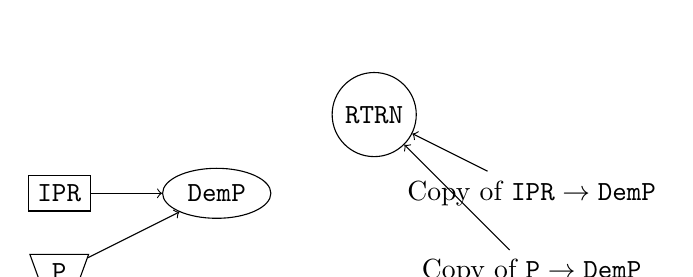
\begin{tikzpicture}
		\node[draw,trapezium,trapezium left angle=-70,trapezium right angle=-70] (P) at (0,0) {\texttt{P}};
		\node[draw] (IPR) at +(0,1) {\texttt{IPR}};
		\node[draw,ellipse] (DemP) at +(2,1) {\texttt{DemP}};
		\node[draw,circle] (Retrn) at +(4,2) {\texttt{RTRN}};
		\node (BlankIPR) at +(6,1) {Copy of $\texttt{IPR}\rightarrow\texttt{DemP}$};
		\node (BlankP) at +(6,0) {Copy of $\texttt{P}\rightarrow\texttt{DemP}$};
		\draw[->] (P) -- (DemP);
		\draw[->] (IPR) -- (DemP);
% 		\draw[->] (DemP) -- (Retrn);
		\draw[->] (BlankIPR) -- (Retrn);
		\draw[->] (BlankP) -- (Retrn);
	\end{tikzpicture}
	\caption{
		Change of the network in Figure \ref{fig:demand1} to simulate demand flowing through potable demand node \texttt{DemP}.
	}
	\label{fig:demand2}
\end{figure}

Note: the arc to the return interceptor is implied, not stored explicitly in \connections, and is required to be the unique return interceptor in the same zone as the potable demand.


\section{Building the constraint matrix}
\label{sec:A}

\subsection{Sub-matrices}
\label{ssec:submatrices}

The constraint matrix constructed by \buildA\ covers all time periods of the problem, and is composed of three sub-matrices: \A, \Ast, and \Alag.
Their basic functions are the following:
\begin{itemize}
	\item \A: Contains all variables in the current time period.
	\item \Ast: Contains storage of currently usable water from previous time periods.
	\item \Alag: Controls the time required for water sent for treatment in previous time periods to become available for use.
\end{itemize}

Each of the three matrices can be further decomposed into sub-matrices.
For example, \A\ can be decomposed as
\begin{equation}
	\A = 
	\left(
	\begin{array}{cccc}
		A &   S & R   & -I \\
		A_\text{ws} & S_\text{ws} & R_\text{ws} &  0 \\
		L &   0 & 0   &  I
	\end{array}
	\right),
	\label{eq:submatrices}
\end{equation}
where $I$ is the identity matrix of appropriate size and $0$ are the matrices of zeros of appropriate size.
The submatrices have dimensions given in Table \ref{tb:submatrices}:
\begin{table}[!h]
	\centering
	\begin{tabular}{|r|c|c|c|c|}
		\hline
		rows $\backslash$ columns& \numArcs & \numStorage & \numRelease & $\numUsers$ \\
		\hline
		\numUsers & $A$           & $S$           & $R$           & $-I$ \\
		\numWS       & $A_\text{ws}$ & $S_\text{ws}$ & $R_\text{ws}$ & $0$  \\
		\numUsers & $L$           & $0$           & $0$           & $I$  \\
		\hline
	\end{tabular}
	\caption{
		Size of each of the sub-matrices in (\ref{eq:submatrices}).
	}
	\label{tb:submatrices}
\end{table}

The dimensions are:
\begin{itemize}
	\item \numUsers: Number of nodes listed as users.
	\item \numArcs: Number of arcs defined in \connections\ (i.e., not including implied arcs).
	\item \numStorage: Number of nodes (groundwater sources and recharge facilities) capable of storing water over time periods.
	\item \numRelease: Number of nodes (surface water sources and waste-water treatment plants) that can release water into the environment.
\end{itemize}

The purpose of each sub-matrix can be determined by it's row and column.
The purposes of the rows:
\begin{itemize}
	\item The first row stores all variables for each node represented as a user in \connections.
	\item The second row stores all variables for each water source node (groundwater or surface water), which are not given as users in \connections.
	\item The third row stores the water lost as it comes into each node listed as a user.
\end{itemize}

The purpose of the columns:
\begin{itemize}
	\item The first column is for flows along arcs.
	\item The second column is for storage decisions.
	\item The third column is for releasing water back into the environment.
	\item The final column connects the movement of water to its transport losses.
\end{itemize}

In sub-matrix \Ast, only the storage columns are nonzero.
Likewise, in sub-matrix \Alag, only the arc columns are nonzero.
In both \Ast\ and \Alag, the identity matrices are replaced with zeros.

\subsection{Combining the sub-matrices for year-long time periods}
\label{ssec:yearlag}

These sub-matrices can be combined in various ways depending on the desired time-step for each period.
The variable \texttt{timeLag} controls the number of time steps per year.
When \texttt{timeLag = 1}, the sub-matrices fit together in a block bi-diagonal form, which for 4 time periods looks like
\[
	\left(
	\begin{array}{cccc}
		\A         &            &            &    \\
		\Ast+\Alag & \A         &            &    \\
					  & \Ast+\Alag & \A         &    \\
					  &            & \Ast+\Alag & \A 
	\end{array}
	\right).
\]

\subsection{Constraint Matrices for other time lags}
\label{ssec:otherlag}

As the code is currently written, the only options are \texttt{timeLag = 1} (for 1-year time steps) and \texttt{timeLag = 12} (for 1-month time steps).
For illustration purposes, the constraint matrix is constructed as follows for \texttt{timeLag = 3}
\[
	\left(
	\begin{array}{ccccc}
		\A    &       &      &      &    \\
		\Ast  & \A    &      &      &    \\
		      & \Ast  & \A   &      &    \\
		\Alag &       & \Ast & \A   &    \\
		      & \Alag &      & \Ast & \A
	\end{array}
	\right).
\]
That is, the sub-matrix \Alag is \texttt{timeLag} columns to the left of sub-matrix \A.
Note that for \texttt{timeLag = 1} the matrices \Ast\ and \Alag\ will overlap, and thus are added together.

\subsection{Loss Factors and Variables}
\label{ssec:loss}

Loss variables, in the $L$ sub-matrix of \A\ and \Alag, store the amount of water lost as the flow travels from the source to the user.
Loss variables (and constraint rows) are named after the user nodes, with a suffix \texttt{-Loss} or \texttt{-loss} added, depending on whether the loss is the standard amount or not.
The standard amount of loss is $1\%$, and is applied to all arcs by default.
Exceptions are as follows:
\begin{enumerate}
	\item Arcs leaving dummy nodes are not subject to loss.
	\item Arcs coming into a recharge facility from either a waste-water treatment plant or a surface water source are not subject to loss.
	\begin{enumerate}
		\item Note: these are the only types of arcs entering a recharge facility in my connections matrices.
				Perhaps the code could be changed to have no loss for any arcs entering a recharge facility.
	\end{enumerate}
	\item Arcs coming into a waste-water treatment plant from either another waste-water treatment plant or a water treatment plant have a $5\%$ loss to solids.
	\begin{enumerate}
		\item Note: Return interceptors can also connect to waste-water treatment plants, and these arcs are subject to the standard loss.
	\end{enumerate}
	\item Arcs coming into recharge facilities from previous time periods have a $3\%$ loss due to evaporation.
\end{enumerate}

There is a potential instability in the code here.
Loss variables are characterized as standard or not based on the user node.
However, some users (WWTPs and potable/non-potable users) may have arcs of both standard and non-standard loss coming into them.
This may make the classification of some loss variables arbitrary.
This may not be a problem, but it should be kept in mind.

\section{Inputs File \inputs}

The second file, containing the cost vector, variable lower and upper bounds, and right hand side vector, is \inputs.
The file is largely self-explanatory, but there is one important catch:
\textbf{There is no consistency checking in the MATLAB code}.
The variables and constraints must be specified in exactly the order that they are read in MATLAB, because the code does not compare the internal names of the variables with the names supplied in the spreadsheet.

\end{document}